\chapter{2DJ Estimation for Pure Shift NMR}
\label{chap:cupid}
Two key features of the \ac{NMR} experiment for which improvements are
constantly being sought are sensitivity and resolving power. There are numerous
means of enhancing sensitivity, such as the use of magnets with higher field
strengths~\cite{Maeda2019} (sensitivity $\propto B_0^{\nicefrac{3}{2}}$) and
cryogenic probes~\cite{Kovacs2020}, as well as simply
increasing the number of scans (sensitivity $\propto \operatorname{NS}^{\nicefrac{1}{2}}$)\label{corr:ns}.
However, few means of achieving better resolution exist beyond increased field
strengths (resolution $\propto B_0$), and ensuing that a homogeneous magnetic
field is used through the use of shimming. Significant interest has therefore
been given to the development of techniques which generate broadband homodecoupled
(\emph{pure shift}) spectra, in which the effects of homonuclear scalar
couplings are absent from the data. While often valuable for structural
assignment purposes, the influence of scalar couplings can lead to spectra
which are too crowded for meaningful insights to be gleaned. While it is
commonplace to decouple heteronuclear couplings at the point of \ac{FID}
acquisition~\cite{Shaka1983a, Shaka1983b,Shaka1985}, homonuclear decoupling is
far more challenging. At the time of writing, there are a number of approaches
for acquiring pure shift spectra; the most popular modern approach
involves running a suitable \ac{2D} pulse sequence, and concatenating the initial
sections of each \ac{FID}, in a process referred to as
``chunking''~\cite{Meyer2013,Adams2014,Zangger2015}. The key drawback of all of
these techniques is that the resultant pure shift signal is considerably less
sensitive relative to a standard pulse-acquire experiment, since only a
fraction of the available spin magnetisation contributes to that which is
incorporated into the dataset.

In this chapter, a method for deriving pure shift spectra indirectly via the
estimation of \ac{2DJ} datasets is presented, which has been named
\acfi{CUPID}. It is illustrated that by extracting the parameters which
describe a \ac{2DJ} dataset, a pure shift spectrum with desirable
absorption-mode lineshapes can be produced without the signal loss associated
with experimental pure shift methods.

\section{Pure Shift \acs{NMR}}

In this section, a survey of some of the most prominent procedures for
producing pure shift spectra are presented.

\subsection{The \acs{2DJ} Experiment}
The \ac{2DJ} experiment\cite{Aue1976, Morris2009} provided the first means of
achieving pure shift spectra. It has a simple pulse sequence:
\[
    \ang{90} \xrightarrow{\nicefrac{\tone}{2}} \ang{180} \xrightarrow{\nicefrac{\tone}{2}} \ttwo.
\]
After excitation of magnetisation onto the transverse plane, the indirect
dimension evolution consists of a spin echo, with acquisition following
immediately afterwards. Fourier transformation in both dimensions leads to a
spectrum in which only scalar couplings contribute in $\Fone$, as the chemical
shifts are refocussed by the spin echo, while both scalar couplings and
chemical shifts contribute in $\Ftwo$.  \Iac{FID} generated by the \ac{2DJ}
experiment is hypercomplex, taking the form of \cref{eq:general-fid} with
$D=2$ and $\zeta^{(1)} = \exp(\iu\cdot)$, i.e.
\begin{equation}%
    \begin{split}%
        y_{\none,\ntwo} =
        &\sum_{m=1}^{M} a_m \exp(\iu \phi_m)
            \exp\left(\left(2 \pi \iu \fonem - \etaonem\right) \none \Dtone\right) \times \\
        &\exp\left(\left(2 \pi \iu  \left(\ftwom - \foff\right)
            - \etatwom\right) \ntwo \Dttwo\right)
            + w_{\none,\ntwo}.
    \end{split}%
    \label{eq:jres-fid}
\end{equation}%
The transmitter offset term has been neglected in the indirect dimension, since
chemical shift evolution does not occur.
For each signal in the \ac{FID}, the indirect- and direct-dimension
frequencies are intimately linked. Consider a \ac{2DJ} dataset generated by a
spin system with $S$ distinct spins. The signals giving rise to a particular
spin $s \in \lbrace 1, \cdots, S \rbrace$ form a grouping $G_s
\subset \lbrace 1, \cdots, M \rbrace$. All of the signals in $G_s$
have (angular) frequencies given by
\begin{subequations}
    \begin{gather}
        2 \pi \fonem = \Updelta \omega_m,\\
        2 \pi \ftwom = \omega_{0,s} + \Updelta \omega_m,
    \end{gather}
    \label{eq:f1-f2-2dj}
\end{subequations}
$\forall m \in G_s$, where $\omega_{0,s}$ is the Larmor frequency of
the spin, and $\Updelta \omega_m$ is the displacement
of the signal from $\omega_{0,s}$, as a result of J-couplings\footnote{
    $\Updelta \omega_m$ will be a linear combination of all the scalar
    couplings associated with the spin giving rise to the signal, with all the
    coefficients being $\pm \nicefrac{1}{2}$.
}. Due to the relationship between the direct- and indirect-dimension
frequencies, all signals which are part of the same multiplet lie along
a line which bisects (i.e. makes a \ang{45} angle with) both the $\Fone$ and
$\Ftwo$ axes, as depicted in \cref{fig:jres_spectrum}.a.
\begin{figure}%
    \centering%
    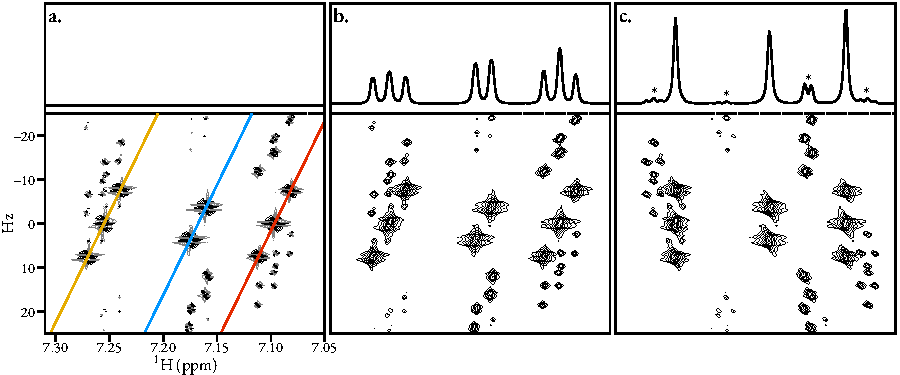
\includegraphics{jres_spectrum/jres_spectrum_new.pdf}%
    \caption[
        Region of a \acs{2DJ} spectrum of strychnine.
    ]
    {%
        Region of a simulated \acs{2DJ} spectrum of strychnine.
        Each panel depicts the spectrum following different processing
        procedures. Below: contour plots of the spectrum. Above: the
        summation of the spectrum along the indirect ($y$) axis.
        \textbf{a.} Spectrum produced by applying sine-bell apodisation
        followed by \ac{FT} in both dimensions.
        Coloured lines denote \ang{45} cross-sections along which the present
        multiplet structures lie.
        \textbf{b.} Magnitude-mode spectrum.
        \textbf{c.} Spectrum generated after application of a \ang{45} shear on
        the magnitude-mode spectrum. Peaks marked with asterisks panel c arise
        from the presence of strong coupling artefacts.
   }%
    \label{fig:jres_spectrum}%
\end{figure}%

One limitation of the \ac{2DJ} experiment is the fact that
spectra with pure absorption lineshapes cannot be produced. This is since, due
to the absence of a mixing period, it is not possible to produce a
complementary pair of phase- or amplitude-modulated \acp{FID}, which are
required to nullify dispersive contributions (see
\cref{subsec:mulitdim}).
The FT of a \ac{2DJ} \ac{FID} produces a spectrum with phase-twist
peaks (\cref{fig:jres_spectrum}.a). As with other experiments which
produce hypercomplex signals, such as \ac{COSY}, the data is conventionally
displayed in ``magnitude-mode'' (\cref{fig:jres_spectrum}.b) in which the
absolute value of each point in the spectrum is plotted.
A pure shift spectrum is generated from the \ac{2DJ} spectrum by performing a
\ang{45} shear\,---\,often referred to as a tilt\,---\,on the spectrum array,
leading to the separation of chemical shifts and scalar couplings onto
orthogonal axes (\cref{fig:jres_spectrum}.c). Each slice through the
direct dimension of the \ac{2DJ} spectrum is subjected to a right circular
rotation such that
\begin{subequations}
    \begin{gather}
        s_{\none,\ntwo}^{\text{tilt}} =
            s_{\none,n^{(2)\prime}},\\
        n^{(2)\prime} = \left(\ntwo + \left\lfloor
                \frac
                    {\fswone \Ntwo\vpsub{\mathrm{sw}}}
                    {\fswtwo \None\vpsub{\mathrm{sw}}}
                \left(
                    \frac{\None\vpsub{\mathrm{sw}}}{2} - \none
                \right)
            \right\rceil
        \right) \bmod \Ntwo.
    \end{gather}
\end{subequations}
This achieves the mapping $s\left(\Fone,\Ftwo\right) \rightarrow s(\Fone, \Ftwo
- \Fone)$, which leads to a spectrum in which all peaks arising from a
given spin reside at the same direct-dimension frequency. The
effectiveness of the shear is maximised when both $\nicefrac{\fswtwo}{\fswone}$
and $\nicefrac{\Ntwo}{\None}$ are powers of 2\note{check this}. Summing the
sheared spectrum along $\Fone$ leads to the pure shift spectrum.
If the spectrum wasn't in magnitude-mode, shearing and summing would lead to
the absorptive and dispersive components of the spectrum cancelling each other
out, such that a vector of noise would be obtained.
With a magnitude-mode spectrum, the process leads to undesirable pure shift
spectra with broad ``wings'' on account of the presence of dispersive
character, and non-linearities. These effects can be suppressed by appropriate
processing to make the FID envelope symmetric in both dimensions, such as with
sine-bell apodisation or pseudo-echo reshaping\cite{Bax1981}, though this
results in a significant reduction in sensitivity being incurred, along with
distortions in relative peak amplitudes.

Another feature which limits the effectiveness of the \ac{2DJ} experiment to
produce pure shift spectra are
\emph{strong coupling artefacts}\footnote{
    As stressed in \cite{Thrippleton2005}, these are not strictly artefacts,
    but rather genuine signals, which are expected to be present in the
    \ac{2DJ} dataset. Despite this, the term is widespread in the literature.
},
which arise due to mixing effects induced by the \ang{180} pulse in the
\ac{2DJ} sequence\cite{Wider1983,Thrippleton2005}. Examples of these are seen
in the spectra of \cref{fig:jres_spectrum}, on account of the three spins
giving rise to the signals seen being strongly coupled. These artefacts always
have direct-dimension frequencies which match those of the conventional signals
in the spectrum\,---\,a feature which will be exploited in the \ac{CUPID}
procedure\,---\,however they do not lie along the same \ang{45} cross
sections. As a result, the final spectrum produced by shearing and summing will
feature extra low intensity signals that do not agree with the chemical shift
of a particular spin (see peaks marked with asterisks in
\cref{fig:jres_spectrum}.c).

\subsection{The \acl{ZS} Method}
\label{subsec:ZS}
Zangger and Sterk introduced a pulse sequence element which achieves
\emph{slice-selective excitation}, by applying a low \ac{RF} power \ang{180}
pulse\footnote{Conventionally, a R-SNOB pulse is used\cite{Kupce1995}.} in the
presence of a \ac{PFG} along the $z$-axis\cite{Zangger1997}. Such an element
excites a
given spin only in a narrow range of heights in the sample, as the \ac{PFG}
induces a shift in resonance frequency according to $\Updelta \omega(z) = \gamma
gz$, where $g$ is the magnitude of the \ac{PFG}. By placing a hard
\ang{180} pulse adjacent to the selective pulse, the
``active'' spin in a given slice is rotated by \ang{360} (i.e. no net
rotation), while all other (``passive'') spins are only rotated by \ang{180}.
Placing such a element in the middle of the $\tone$ evolution therefore
achieves refocussing of the J-couplings associated with the active
spin\cite{Aguilar2010}. In order to achieve effective decoupling of any given
pair of spins, it is necessary that the bandwidth of the selective π-pulse is
smaller than the difference in their Larmor frequencies. However, with more
selective pulses, a smaller proportion of the available spin magnetisation will
contribute to the final FID, and hence sensitivity will be diminished
\footnote{
    The reduction in sensitivity is $\propto \nicefrac{\Updelta F}{\gamma g l_z}$,
    where $\Updelta F$ is the selective pulse bandwidth, and $l_z$ is the length of
    the sample lying within the receiver coil ($\approx
    \qty{1.5}{\centi\meter}$).
}.
Therefore a trade-off exists between effective decoupling of all spins, and
achieving the greatest sensitivity possible. In the case of strong coupling,
the \ac{ZS} method tends to perform poorly relative to other options for this
reason. The \ac{ZS} element has been utilised in order to generate \ac{2DJ}
datasets comprising phase-modulated pairs, enabling the generation of pure
absorption-mode spectra\cite{Pell2007}. Pure shift spectra with far more
desirable lineshapes can be achieved relative to using a typical magnitude-mode
spectrum \ac{2DJ}, though with a significant loss of sensitivity.

\subsection{The \acs{BIRD} Method}
The \ac{BIRD} pulse sequence element\cite{Garbow1982,Bax1983} also takes
advantage of the idea of selectively inverting passive spins, while leaving
active spins unaffected.
However the active spins are those which are directly bound to a low natural
abundance
heteronucleus, with the two most common heteronuclei used being
\textsuperscript{13}C (1.1\% abundance) and \textsuperscript{15}N (0.37\%
abundance).
The passive spins are those bound to far more abundant nucleus (i.e.
\textsuperscript{12}C or \textsuperscript{14}N). The reduction in sensitivity
of the experiment relative to a full-sensitivity experiment is therefore known
and constant across samples. In scenarios where strong coupling exists, \ac{BIRD} can
achieve improved sensitivity over \ac{ZS}, since with the latter a very weak
selective pulse would be required to ensure it is of a sufficiently small
bandwidth. The \ac{BIRD} method is particularly attractive in scenarios where
the sensitivity penalty due to the involvement of a low-abundance nucleus has
already been paid, for example in sequences where an \ac{INEPT} element is
present\cite{Paudel2013}. One of \ac{BIRD}'s primary drawbacks is the fact that
geminal protons (i.e. protons bound to the same heteroatom) cannot be decoupled
from each other, since such protons are always in the same subset of either
active or inactive nuclei. Doublets rather than singlets will arise in such
cases.

\subsection{\acs{PSYCHE}}
\label{subsec:psyche}
The most recent major development in pure shift spectroscopy is the \ac{PSYCHE}
experiment\cite{Foroozandeh2014,Foroozandeh2018}.
\note{Description... Element, How it works (very simple), Effectiveness}

With \ac{PSYCHE}, the proportion of active and passive spins is
dependent on the flip angle of the chirp pulses; for a
\ac{PSYCHE} element featuring chirp pulses with flip angles $\beta$, the
proportions of are $\cos^2 \beta$ and $\sin^2 \beta$, respectively.

The \ac{PSYCHE} element has also been employed in conjunction with the \ac{2DJ}
experiment in order to produce spectra which already feature orthogonal
separation of the chemical shifts and couplings along the two frequency
axes\cite{Foroozandeh2015,Kiraly2017}. Being a 3D experiment, the
\ac{PSYCHE}-\ac{2DJ} requires long experiment times (typically tens of hours)
in order to produce a spectrum with well-resolved multiplet structures in the
indirect dimension.

\subsection{Pure shift spectra from 2DJ estimation}
\note{Mandelstahm?}

Beyond specialised pulse sequences, procedures based on the estimation of
\ac{2DJ} datasets have also been developed to achieve broadband homodecoupling.
Nuzillard introduced \ac{ALPESTRE}\cite{Nuzillard1996,Martinez2012}, in which
the parameters of each indirect-dimension FID are estimated using \ac{LPSVD},
such that a set of parameters $\symbf{\Theta} \in \mathbb{R}^{\Ntwo
\times 4M}$ is generated.
\begin{equation}
    \symbf{\theta}_{\ntwo} =
    \begin{bmatrix}
        \bda_{\ntwo}\T &
        \bdphi_{\ntwo}\T &
        \bdf_{\ntwo}\T &
        \bdeta_{\ntwo}\T
    \end{bmatrix}\T.
\end{equation}
The parameters generated are used to propagate each FID backward into
$-\tone$, producing a ``full-echo'':
\begin{equation}
    \begin{split}
        y^{\text{full}}_{\none,\ntwo} = \sum_{m=1}^{M}
            a_{\ntwo,m}
            \exp(\iu \phi_{\ntwo,m})
            \exp\left(\left(2 \pi \iu f_{\ntwo,m} \none
            -\eta_{\ntwo,m}  \left\lvert \none \right\rvert \right)\Dtone\right), \\
        \forall \none \in \lbrace -\None + 1, \cdots, 0, \cdots, \None - 1 \rbrace,\ \forall \ntwo \lbrace 0, \cdots, \Ntwo - 1 \rbrace.
    \end{split}
    \label{eq:full-echo}
\end{equation}
\ac{FT} of \cref{eq:full-echo} generates a spectrum whose real component
comprises absorption-mode
Lorentzian character in both dimensions. This opens up the means of producing
pure-shift spectra from the \ac{2DJ} experiment with sharp lineshapes and
without signal loss. A similar approach proposed by Mutzenhardt et al.
instead constructs full echoes via \ac{LP} of each direct-dimension
\ac{FID}, and generates a full echo by propagating into
$-\ttwo$\cite{Mutzenhardt1999}.



\section{Methodology}
\ac{CUPID}, a new method developed for pure shift \ac{NMR}, fits into the category
of techniques which utilise \ac{2DJ} estimation. In this section, a description
of it is given.

\subsection{The Estimation Routine}
Recall the assumption that a \ac{2DJ} \ac{FID} takes the functional form
of \cref{eq:jres-fid} (\cpageref{eq:jres-fid}). The primary steps involved in
estimating a \ac{2DJ} dataset, for a given spectral region of interest, are:
\begin{enumerate}
    \item Generation of a frequency-filtered sub-\ac{FID} corresponding to
        the region of interest (\textit{vide infra}:
        \cref{subsec:jres-filtering}).
    \item Prediction of the sub-\ac{FID}'s model order, either by applying the
        \ac{MDL} on the first increment in the direct dimension\footnote{
            The first increment of a \ac{2DJ} experiment, for which $\tone =
            \qty{0}{\second}$, effectively takes the same form as an \ac{FID}
            derived from a pulse-acquire experiment.
        } (\cref{subsec:model-order}, \cpageref{subsec:model-order}) or
        by manually specifying a value.
    \item Generation of an initial parameter estimate using the \ac{MMEMPM}
        (\cref{subsec:mmempm}, \cpageref{subsec:mmempm}).
    \item Subjection of the initial parameter estimate to phase
        variance-regularised \ac{NLP} (\cref{sec:nlp}, \cpageref{sec:nlp}).
\end{enumerate}
Instead of estimating successive \ac{1D} \acp{FID}, as proposed by
Nuzillard and Mutzenhardt \emph{et~al.}, \ac{2DJ} sub-\acp{FID} are considered
holistically; a number of benefits are realised because of this.
First, multiplet structures which heavily overlap in a
conventional \ac{1D} dataset can become separated in the \ac{2DJ} dataset,
assuming that the Larmor frequencies of the relevant spins are sufficiently
different.
Accurate resolution of the \ac{FID}'s constituent signals in more crowded spectral
regions is far more likely to be successful with a full \ac{2D} estimation as a
result.
On top of this, there is an additional resolution advantage relative to the
estimation of \emph{direct} dimension \ac{1D} \acp{FID}. Due to the presence of a spin
echo during $\tone$, signal damping effects caused by field inhomogeneities are
nullified, such that damping is dictated solely by transverse relaxation
($T_2^{\vphantom{*}}$). However, during $\ttwo$, the influence of field
inhomogeneities is not
corrected, such that damping occurs at a faster rate, characterised by $T_2^*$
(see \cref{fn:t2-star} in \cref{sec:seq}, \cpageref{fn:t2-star}).
As such, multiplet structures in the indirect dimension exhibit better
resolution (assuming $\nicefrac{\fswone}{\None}$ and
$\nicefrac{\fswtwo}{\Ntwo}$ are comparable).
A further benefit comes with having access to the frequencies of
signals in \emph{both} dimensions, since this opens up the opportunity to group
together those which belong to the same multiplet, as will be discussed in
\cref{subsec:mp-selection}.
Similar information can be obtained
by extracting cross-sections of a sheared magnitude-mode \ac{2DJ} spectrum at
appropriate values of $F^{(2)}$, though the lineshapes of peaks suffer from the
undesirable characteristics described above.

As was mentioned in \cref{subsec:model-order} (\cpageref{subsec:model-order})
applying the \ac{MDL} on a \ac{2D} \ac{FID} is time-consuming,
since a complete \ac{SVD} computation on the
very large block-Hankel matrix $\symbf{E}_{\symbf{Y}}$ would need to be
performed.
Assuming that the spectral region being considered is not too
crowded, applying the \ac{MDL} on the first direct-dimension \ac{FID} can
return reasonable estimates of $M$ at a far smaller computational cost. For
particularly crowded regions, resorting to a manual specification of model
order by inspecting the \ac{2DJ} spectrum is the best solution currently
available.
An interesting benefit is sometimes realised when the \ac{1D} \ac{MDL} is
used for model order selection.
As has been discussed above, the presence of strong coupling artefacts in the
\ac{2DJ} dataset leads to additional nuisance peaks appearing in pure shift spectra
produced by the shear-and-project approach. Exactly the
same phenomenon would occur when parametric estimation is employed, assuming
that the strong coupling artefacts are incorporated into the parameter
set. However, since the
artefacts have direct-dimension frequencies which are identical to those of
first-order signals in the dataset, it is incredibly challenging to resolve
these using the \ac{1D} \ac{MDL}. Therefore, the \ac{MDL} is often
found to predict a model order which agrees with the number of first-order
signals, rather than the \emph{true} number of signals in the \ac{FID}. As the
\ac{MMEMPM} generates a parameter estimate based on the $M$ most significant
components of in dataset, the more intense first-order signals are expected to
be quantified, whereas the weaker strong coupling artefacts will be neglected.
It should be noted that this concept is not infallible, though it has been
observed on a number of occasions. There are instances where strong coupling
artefacts are incorporated into the estimation result, either because the
prediction of $M$ was excessive, or certain artefacts possess particularly
large amplitudes; examples of these situations will be seen later.

\subsection{The \ang{-45} Signal}
\begin{figure}
    \centering
    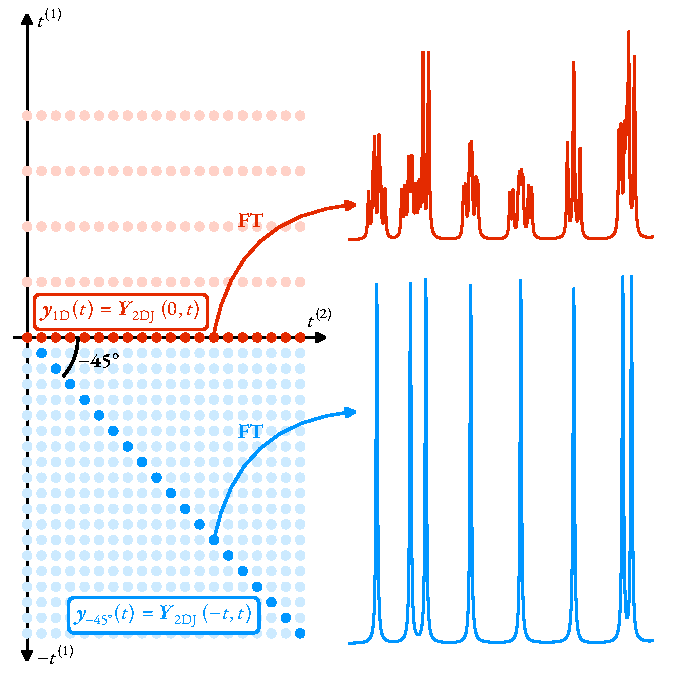
\includegraphics{neg_45_signal/neg_45_signal.pdf}
    \caption[
        The reasoning behind the name ``\ang{-45}
        signal'', which is used to generate pure shift spectra as part of
        \acs{CUPID}.
    ]{
        The reasoning behind the name ``\ang{-45}
        signal'', which is used to generate pure shift spectra as part of
        \ac{CUPID}. The pale red
        dots denote
        a typical \ac{2DJ} \ac{FID}, where
        the amount and rate of sampling in the direct dimension is greater than
        in the indirect dimension (i.e. $\None \ll \Ntwo$ and $\fswone \ll
        \fswtwo$). The bright red dots correspond to the first direct-dimension
        signal $\bY_{\text{2DJ}}(0,\ttwo)$, which has the same form as
        \iac{FID} from a pulse-acquire experiment. A hypothetical signal
        generated by propagating the \ac{FID} into $-\tone$, with the same rate
        of sampling in both dimensions, is denoted with pale blue dots. Taking
        the diagonal of this signal, such that it forms a \ang{-45} angle with the
        $\ttwo$ axis\,---\,the convention of angles being defined through an
        anticlockwise rotation starting on the $\ttwo$-axis has been applied
        here\,---\,yields an \ac{FID}
        $\by_{\ang{-45}}$  which is
        homodecoupled. Note that there is a slight discrepancy
        between \cref{eq:neg-45} and this description, in that the
        indirect dimension damping factors $\bdetaone$ are neglected in the
        former case.
    }
    \label{fig:neg-45}
\end{figure}
The \ac{2DJ} estimation routine yields the parameter vector $\bth \in
\mathbb{R}^{6M}$. With
knowledge of the frequencies and damping factors in both dimensions, it is
possible to generate \iac{FID} which will produce a pure shift spectrum
directly, rather proceeding via the full-echo approach of Nuzillard and
Mutzenhardt \emph{et~al}.
The desired synthetic \ac{FID} produced is named the \emph{\ang{-45} signal}
$\symbf{y}_{\ang{-45}} \in \mathbb{C}^{\Ntwo}$:
\begin{equation}
    y_{\ang{-45},\ntwo} =
        \sum_{m=1}^{M} a_m \exp (\iu \phi_m)
        \exp\left(\left(2 \pi \iu \left(\ftwo_m - \fone_m - \foff\right)
                - \etatwo_m
            \right) \ntwo \Dttwo
        \right),
    \label{eq:neg-45}
\end{equation}
with the reasoning behind the name provided by \cref{fig:neg-45}.
The \ang{-45} signal
takes the form of a conventional \ac{1D} \ac{FID},
except that the frequency of each oscillator, which would be $\ftwo_m$ in a
pulse-acquire experiment,
is replaced with $\ftwo_m - \fone_m$. In the \ang{-45} signal, oscillators
belonging to the same multiplet $s$ will all provide a contribution to the
\ac{FID} with the frequency $f_{0,s}$.
Assuming that the parameters associated with the \ac{2DJ}
\ac{FID} are accurately determined, a pure shift spectrum with sharp
absorption-mode lineshapes and no loss of signal can be generated by this approach.

\subsection{Filtration of \ac{2DJ} Data}
\label{subsec:jres-filtering}
Unlike the direct dimension, which can often comprise sparsely distributed
peaks in the Fourier domain, the indirect dimension of \ac{2DJ} datasets tends
to be densely populated since all multiplet structures are centered at
\qty{0}{\hertz}, and rarely span beyond $\pm \qty{50}{\hertz}$. As such,
the generation of frequency-filtered sub-\acp{FID} is limited to
the direct dimension in \ac{2DJ} estimation.
The filtering procedure applied to \ac{2DJ} data is an extension of that
for \ac{1D} data described in \cref{sec:filtering} (\cpageref{sec:filtering}):
\begin{enumerate}
    \item The array $\symbf{Y}_{\text{VE}} \in \mathbb{C}^{\None \times 2
        \Ntwo}$, is constructed, which contains the \ac{VE} of each
        direct-dimension \ac{FID}, i.e. each row of the array is given by
        \begin{equation}
            \begin{gathered}
            \by_{\text{VE},\none} =
                \begin{bmatrix}
                    \Re\left(y_{n^{(1)}, 0}^{\vphantom{*}}\right) &
                    y_{n^{(1)}, 1}^{\vphantom{*}} &
                    \cdots &
                    y_{n^{(1)}, \Ntwo - 1}^{\vphantom{*}} &
                    0 &
                    y_{n^{(1)}, \Ntwo - 1}^* &
                    \cdots &
                    y_{n^{(1)}, 1}^*
                \end{bmatrix},\\
                \forall n^{(1)} \in \lbrace 0, \cdots, N^{(1)} - 1 \rbrace.
            \end{gathered}
        \end{equation}
    \item $\symbf{Y}_{\text{VE}}$ is subjected to \ac{FT} along the direct
        dimension to produce the spectrum  $\symbf{S}_{\text{VE}}$
        (\cref{fig:jres-filtering}.a); this has an imaginary component of
        zeros.
    \item A super-Gaussian $\symbf{G} \in \mathbb{R}^{\None \times 2 \Ntwo}$ is
        constructed
        (\cref{fig:jres-filtering}.b):
        \begin{equation}
            \symbf{G} = \symbf{1} \otimes \symbf{g}^{(2)},
        \end{equation}
        where $\symbf{1} \in \mathbb{R}^{\None}$ is a vector of ones, and
        $\symbf{g}^{(2)} \in \mathbb{R}^{2\Ntwo}$ is a super-Gaussian vector
        given by \cref{eq:super-Gaussian-onedim}
        (\cpageref{eq:super-Gaussian-onedim}).
    \item A matrix of additive noise is generated by extracting the variance
        $\sigma^2$ of a direct-dimension strip of $\symbf{S}_{\text{VE}}$ which
        is devoid of peaks, and generating an array $\symbf{W}_{\sigma^2} \in
        \mathbb{R}^{\None \times 2 \Ntwo}$ with values independently sampled
        from $\mathcal{N}(0, \sigma^2)$ (\cref{fig:jres-filtering}.c).
    \item The spectrum is filtered (\cref{fig:jres-filtering}.d):
        \begin{equation}
            \widetilde{\symbf{S}}_{\text{VE}} = \symbf{S}_{\text{VE}} \odot
            \symbf{G} + \symbf{W}_{\sigma^2} \odot (\symbf{1} - \symbf{G}).
        \end{equation}
    \item $\widetilde{\symbf{S}}_{\text{VE}}$ is subjected to \ac{IFT} and is
        sliced in half in the direct dimension, yeilding the final filtered
        signal $\widetilde{\symbf{Y}}$.
\end{enumerate}
As with the \ac{1D} case, this method can also be extended to
incorporate spectral slicing, acting to reduce the number of points present in
the filtered sub-\ac{FID}.

\begin{figure}
    \centering
    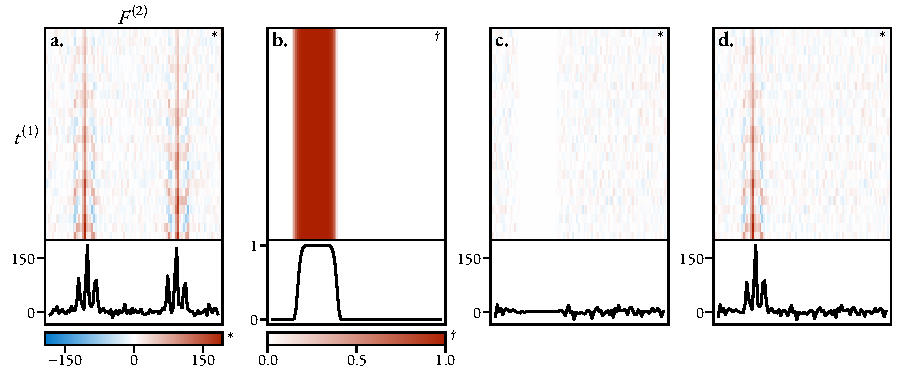
\includegraphics{jres_filtering/jres_filtering.pdf}
    \caption[
        The filtering procedure for \acs{2DJ} data.
    ]
    {
        The filtering procedure for \ac{2DJ} data.
        Each panel consists of a heat-map of the complete \ac{2D} array, as well as
        a plot of the first slice of the array in the direct dimension ($x$-axis).
        \textbf{a.} The spectrum $\symbf{S}_{\text{VE}}$,
        \textbf{b.} Super-Gaussian filter $\symbf{G}$,
        \textbf{c.} Additive noise, attenuated by the super-Gaussian, $\symbf{W}_{\sigma^2} \odot (\symbf{1} - \symbf{G})$,
        \textbf{d.} Filtered spectrum $\widetilde{\symbf{S}}_{\text{VE}}$
        Figures \ref{fig:jres-filtering}.a to \ref{fig:jres-filtering}.d
        are analogous to
        Figures \ref{fig:filtering}.b to \ref{fig:filtering}.e
        for the \ac{1D} case (\cpageref{fig:filtering}).
    }
    \label{fig:jres-filtering}
\end{figure}


\subsection{Multiplet Prediction}
\label{subsec:mp-selection}
\ac{CUPID}'s ability to group oscillators present in a parameter set into
multiplet structures relies on simultaneously knowing both the indirect- and
direct-dimension frequencies of each model oscillator. As has already been
established, for oscillators which are associated with the same multiplet
grouping $G_s$, the quantities $\ftwo_{m_1} - \fone_{m_1}$ and $\ftwo_{m_2} -
\fone_{m_2}$ should be equal ($f{0,s}$) for any pairing  $m_1, m_2 \in
G_s$. An assessment of whether two oscillators belong to the same multiplet can
therefore be made using the following criterion:
\begin{equation}
    \left \lvert
        \left( \ftwo_{m_1} - \fone_{m_1} \right) -
        \left( \ftwo_{m_2} - \fone_{m_2} \right)
    \right \rvert < \epsilon.
\end{equation}
$\epsilon \in \mathbb{R}_{>0}$ is a threshold to account for uncertainty in
the estimation result. A lower bound on $\epsilon$ is the separation between
adjacent points in the better-resolved dimension of the spectrum, i.e.
$\min\left(\nicefrac{\fswone}{\None},
\nicefrac{\fswtwo}{\Ntwo}\right)$.  However, limitations in resolution due to
relaxation-induced signal damping and field inhomogeneities can require
$\epsilon$ to be increased beyond this for effective assignments
to be achieved. \Cref{lst:mp-assign} (\cpageref{lst:mp-assign}) provides a
\Python routine that can be used for multiplet prediction.

There are certain circumstances where it is safe to assume that a
particular oscillator in the estimation result is not associated with a
first-order signal in the dataset;
no oscillator which was derived from a first-order signal will abide by both of
the following:
\begin{enumerate}
    \item The oscillator is not grouped with any other oscillator as part of
        the multiplet assignment.
    \item The magnitude of the indirect dimension frequency of the oscillator
        is appreciably greater than \qty{0}{\hertz}.
\end{enumerate}
If a first-order signal is the only
member of a multiplet grouping, it must be a singlet, and as such it will have
an indirect-dimension frequency of \qty{0}{\hertz}. Oscillators which do agree
with the two points above can be assumed to be related to either strong
coupling artefacts or noise, and can be automatically discarded from the final
parameter estimate.

\correction{
    It is worth mentioning that the procedure of multiplet prediction outlined
    does not naturally allow one to determine the coupling constants associated
    with each spin. With a complete list of the
    frequencies associated with a multiplet structure, the relevant spin's
    coupling network can be predicted. However, it is not guaranteed that the
    estimation routine will extract all frequencies within a multiplet; this is
    particularly so with complex multiplets with significant signal overlap.
    However, it is typically the case that the frequencies extracted by the
    estimation routine can be used as a starting point to manually determine
    the coupling constants.
}\label{corr:coupling-constants}

\section{Results}
\label{subsec:cupid-results}
A number of examples of the application of \ac{CUPID} are now provided.
Initially, a few results are presented on datasets simulated using
\textsc{Spinach}. After this, examples are provided with experimental data. In
a couple of these, comparison of the result acquired using \ac{CUPID} is
made with a spectrum acquired using \ac{PSYCHE}. For details relating to
generation of the datasets, see Sections \ref{sec:simulated-datasets} and
\ref{subsec:cupid-experimental} in the Appendix.

\subsection{``Four Multiplets''}
\label{subsec:four-mp}
\begin{figure}
    \centering
    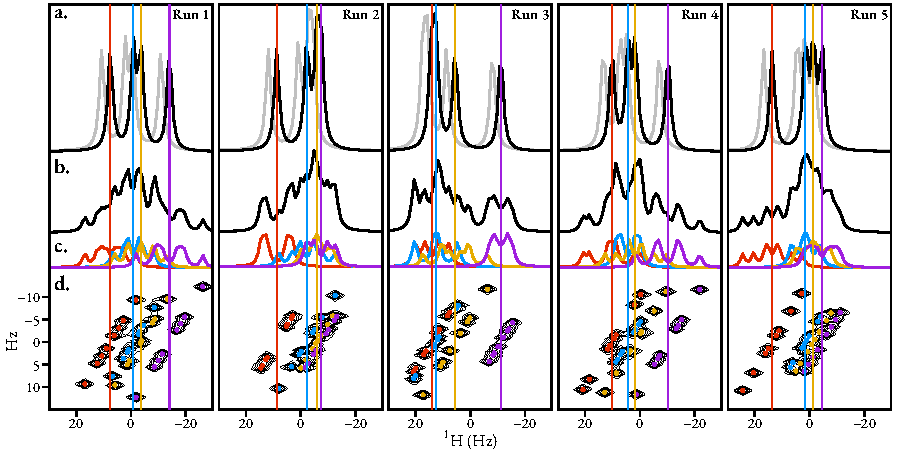
\includegraphics{four_multiplets/four_multiplets}
    \caption[
        The result of applying \acs{CUPID} to 5 instances of simulated
        \acs{2DJ} datasets with 4 heavily overlapping multiplet structures.
    ]{
        The result of applying \ac{CUPID} to 5 instances of simulated \ac{2DJ}
        datasets with 4 heavily overlapping multiplet structures.
        \textbf{a.} Black: pure shift spectrum generated by \ac{CUPID} (via the
        \ang{-45} signal).
        Grey: \ac{1D} spectrum simulated with Spinach, using the same spin
        system as was used to produce the \ac{2DJ} dataset, but with all scalar
        couplings set to \qty{0}{\hertz}. This has been offset slightly for
        clarity.
        \textbf{b.} \ac{1D} spectrum of the dataset, produced using the first
        direct-dimension \ac{FID} in the \ac{2DJ} dataset.
        \textbf{c.} Multiplet structures predicted, using a threshold $\epsilon
        = \nicefrac{\fswtwo}{\Ntwo} \approx \qty{0.98}{\hertz}$.
        \textbf{d.} Contour plot of the \ac{2DJ} spectrum in absolute-value
        mode. Coloured points denote the frequencies of oscillators in the
        estimation result.
        Coloured vertical lines denote the predicted central frequencies of
        each multiplet structure.
    }
    \label{fig:four-multiplets}
\end{figure}
A series of simulated \proton\ \ac{2DJ} datasets were generated such that
within a known region of the spectrum (\SIrange{-30}{30}{\hertz}), four ddd
multiplet structures with significant overlap exist. To achieve this, a
spin-system with 7 spins was formed, with the spins divided into 2 subsets:
\begin{itemize}
    \item Four of the spins (the ``estimated spins'') were assigned random
        resonance frequencies sampled from $\mathcal{U}(\qty{-20}{\hertz},
        \qty{20}{\hertz})$.
    \item The remaining three spins (the ``coupling spins''), were coupled to each
        of the estimated spins, with the values of the couplings randomly
        sampled from $\mathcal{U}(\qty{-10}{\hertz}, \qty{10}{\hertz})$.  The
        coupling spins were given chemical shifts such that they lay far from
        the estimated spins in the spectrum (i.e. their frequencies were $\gg
        \qty{20}{\hertz}$).
\end{itemize}
\ac{AWGN} noise was added to the \ac{FID}, with a target \ac{SNR} of \qty{30}{\deci\bel}.
A filtered sub-\ac{FID} containing only the signals from the estimated spins
was then generated using the filtering procedure described above, with
$l^{(2)}_{\unit{\hertz}} = \qty{30}{\hertz}$,
$r^{(2)}_{\unit{\hertz}} = \qty{-30}{\hertz}$.
The resulting sub-\ac{FID} was expected to comprise 32 ($4 \times
2^3$) oscillators. To assess the estimation procedure's ability, a random
integer from the range $[33, 40]$ was selected as the initial number of
oscillators. Hence, the initial guess from the \ac{MMEMPM} would comprise a
excessive number of oscillators. Due to the severe overlap of the multiplets,
application of the \ac{MDL} on the first direct-dimension signal would be
ineffective and return an under-estimate of the model order. Each \ac{FID} was
subjected to estimation, yielding the result vector $\bthstar$. Spurious
oscillators were checked for, using the criteria outlined above, with the
threshold for multiplet assignment set to the spectral resolution in the direct
dimension: $\epsilon = \nicefrac{f_{\text{sw}}^{(2)}}{\Ntwo}$. If spurious
oscillators were found, these were removed, and \ac{NLP} was run on the updated
set of parameters.

Figure \ref{fig:four-multiplets} illustrates the result achieved for 5 separate
runs of this procedure.
For each \ac{FID} generated, the method was effective at producing an
estimation result with 32 oscillators, as desired, despite the excessive number
that were present in $\bthzero$. Most of the excessive oscillators were purged
from $\bthzero$ through the \ac{NLP} procedure. When spurious oscillators did
remain\footnote{for 2 of the 5 datasets, the result after \ac{NLP} comprised 33
oscillators}, they were then detected when checking for spurious oscillators
and subsequently removed. With simulated examples, it is easy to confirm that
the pure shift spectrum generated using \ac{CUPID} agrees with the expected
pure shift spectrum; it is possible to generate the ``true'' pure shift
spectrum by simulating a pulse-acquire experiment with \textsc{Spinach}, using
a spin system with same chemical shifts, but all scalar couplings set to
\qty{0}{\hertz}.
As seen in panel a of Figure \ref{fig:four-multiplets}, the spectra produced
using \ac{CUPID} agree well with these. Panel c indicates that \ac{CUPID}
effectively resolved the multiplet structures associated with the dataset.

\subsection{Sucrose simulated}
\label{subsec:sucrose-cupid}
\note{Maybe not so impressive? Perhaps try strychnine?}
\begin{figure}
    \centering
    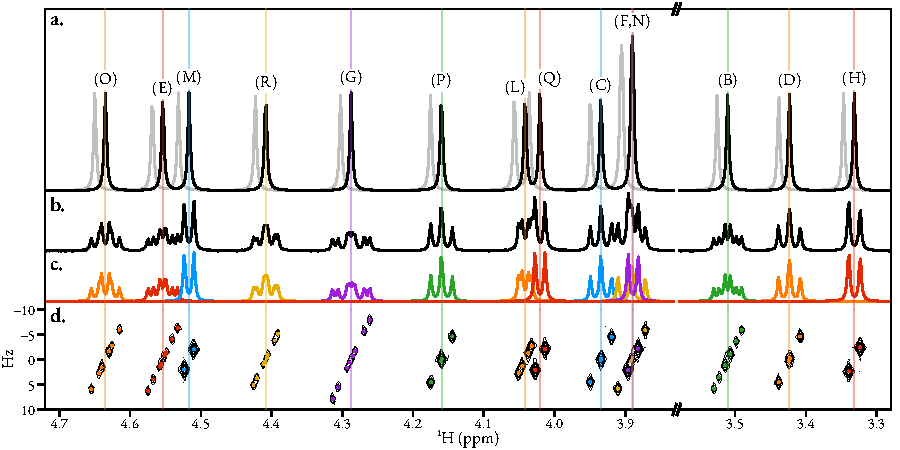
\includegraphics{sucrose_cupid/sucrose_cupid.pdf}
    \caption[
        Application of \acs{CUPID} on a simulated sucrose \acs{2DJ} dataset.
    ]
    {
        Application of \ac{CUPID} on a simulated sucrose \ac{2DJ} dataset.
        \textbf{a.} Black: the spectrum generated from \ac{FT} of the \ang{-45}
        signal. Grey: the spectrum of a simulated dataset with the same
        chemical shifts, with all scalar couplings set to \qty{0}{\hertz}.
        \textbf{b.} Conventional \ac{1D} spectrum.
        \textbf{c.} Multiplet structures assigned ($\epsilon \approx
        \qty{0.27}{\hertz}$).
        \textbf{d.} Contour plot of the absolute value mode \ac{2DJ} spectrum,
        with the locations of assigned oscillators given as coloured points.
    }
    \label{fig:sucrose-cupid}
\end{figure}
As a second example of applying \ac{CUPID} on simulated data, the chemical
shifts and isotropic scalar couplings associated with a
Gaussian\cite{Gaussian03} \ac{DFT} calculation of sucrose in a vacuum
\footnote{
It is well known that isotropic chemical shift calculations using \ac{DFT} are
typically very inaccurate. The resulting spectrum is not typical of sucrose in
the liquid state, though this doesn't really matter for assessing the
performance of \ac{CUPID}.
}
were used to construct a 2DJ dataset. \ac{AWGN} was added with a target
\ac{SNR} of \qty{20}{\deci\bel}. The CUPID procedure was applied to filtered
sub-FIDs such that the signals arising from all 22 spins were considered, though
only the regions of the dataset with the most interesting multiplet structures
are presented in Figure \ref{fig:sucrose-cupid}.

The estimation technique successfully assigned multiplet structures for all 22
multiplets in the dataset, including structures derived from two spins (F \& N)
with a \qty{0.6}{\hertz} difference in resonance frequency, approaching the
spectral resolution in the direct dimension (\qty{0.537}{\hertz}). The
pure-shift spectrum generated via the \ang{-45} signal again showed close
agreement with a 1D spectrum simulated using the same chemical shifts, with
scalar couplings set to \qty{0}{\hertz}. There are particular multiplets where
the number of oscillators fit using the estimation routine was less than the
true number. Examples of this phenomenon are exhibited in the estimates of the
multiplets for spins B \& O, which are both ddd structures. The scalar
couplings involved meant that certain oscillators were
of such similar frequencies that they were separated by significantly less than
the spectral resolution, and thus resolving these was unrealistic. For
example, there are two pairs of peaks in the spin-B multiplet which lie only
\qty{0.085}{\hertz} apart. Under-fitting in this case had a negligible impact
on the final pure shift spectrum. However there are circumstances which will be
seen in the experimental examples below where more blatant cases of under-fitting
lead to the generation of peaks in the pure shift spectrum which are noticeably
broadened.

\subsection{Quinine}
\begin{figure}
    \centering
    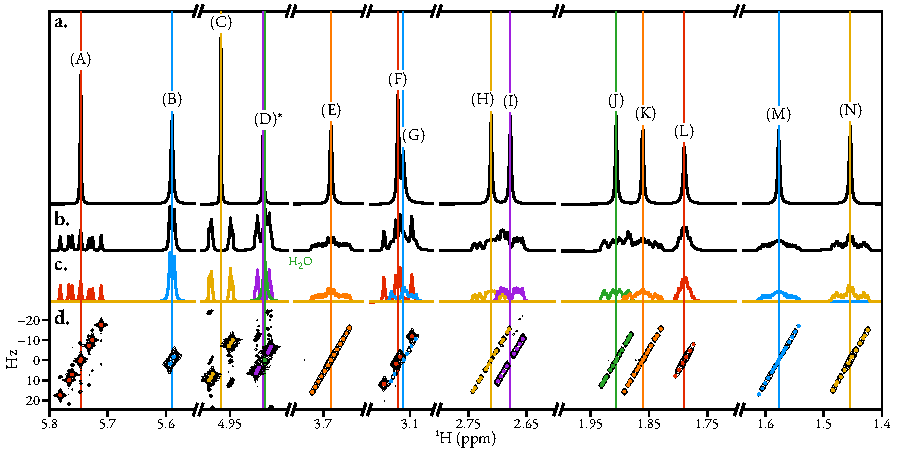
\includegraphics{quinine_cupid/quinine_cupid.pdf}
    \caption[
        Application of \acs{CUPID} on the non-aromatic regions of a quinine
        \acs{2DJ} dataset.
    ]{
        Application of \ac{CUPID} on the non-aromatic regions of a quinine
        \ac{2DJ} dataset.
        \textbf{a.} The spectrum generated from \ac{FT} of the \ang{-45}
        signal, with the signal arising from H\textsubscript{2}O (green, close
        to \qty{4.9}{\partspermillion} neglected).
        \textbf{b.} Spectrum of the first direct-dimension signal in the
        \ac{2DJ} \ac{FID}.
        \textbf{c.} Multiplet structures assigned ($\epsilon =
        \nicefrac{\fswtwo}{\Ntwo} \approx \qty{0.92}{\hertz}$).
        \textbf{d.} Contour plot of the absolute value mode \ac{2DJ} spectrum,
        with the locations of assigned oscillators given as coloured points.
    }
    \label{fig:quinine-cupid}
\end{figure}

Figure \ref{fig:quinine-cupid} illustrates the result of applying \ac{CUPID} on
a dataset generated from a sample comprising quinine (Figure
\ref{fig:structures}.a) in CD\textsubscript{3}OD,
with all signals arising from non-aromatic protons considered. The method
successfully generated a
pure shift spectrum with distinct peaks for each \textsuperscript{1}H
environment. This example also highlights an added benefit of using \ac{CUPID};
it provides the opportunity to suppress ``nuisance'' signals in the pure shift
spectrum. In this
example, an intense, broad singlet at around \qty{4.89}{\partspermillion}
was detected (see the green peak at this frequency in panel c).
The singlet was due to the presence of water in the sample and was a hindrance
due to it overlapping heavily with the multiplet structure corresponding to
spin (D). To obtain a clean singlet for spin (D) in the pure shift spectrum, the
oscillator corresponding to the water signal was simply neglected from
the parameter set used to generate the \ang{-45} signal. This concept of neglecting
nuisance signals through post-processing has been employed extensively, with
the most prominent use case being solvent suppression. The most
significant component in the data (assumed to be the solvent peak), is
determined through \ac{SVD} or some other approach, and is automatically
subtracted from the \ac{FID}\cite{Zhu1997}.
In this case, the water signal is not automatically purged from the parameter
set to construct the final pure shift spectrum, but a knowledgeable user would
be able to locate the water signal, determine that it is undesirable to include
in the pure shift spectrum, and neglect it.


As eluded to already, a few of the peaks in the pure-shift spectrum are rather
broad on account of the estimation routine under-fitting the relevant multiplet
structure. The most notable example of this phenomenon in the quinine example
comes from the peak for spin (G), where close proximity with the spin (F)
multiplet has likely compounded the task of accurately estimating the relevant
oscillators. With fewer oscillators than the true number of contributing signals
fitting a given multiplet structure, the \ac{NLP} routine will compensate by
giving the oscillators it does have at its disposal large amplitudes and
damping factors, so that they can reasonably fit multiple similar-frequency
signals. This behaviour is also exhibited by the multiplet for spin (B),
which comprises two pairs of very close signals in a dd structure. A single
oscillator is fit to each pair of signals, culminating in a broadened pure
shift peak. While linewdiths are affected by under-fitting hard-to-resolve
multiplets, the integrals of the pure shift peaks are not typically perturbed
significantly. \note{COMPUTE INTEGRALS}

\subsection{Camphor}
\begin{figure}%
    \centering%
    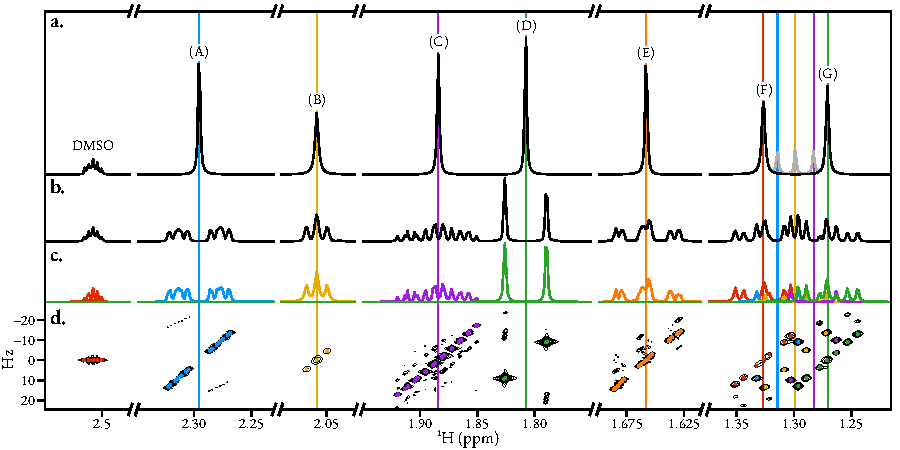
\includegraphics{camphor_cupid/camphor_cupid.pdf}%
    \caption[
        Application of \acs{CUPID} on a camphor dataset.
    ]{
        Application of \acs{CUPID} on camphor \ac{2DJ} dataset.
        \textbf{a.} Black: the spectrum generated from \ac{FT} of the \ang{-45}
        signal. Oscillators associated with strong coupling artefacts between
        spins (F) and (G) were neglected. Grey: spectrum generated without
        neglecting oscillators associated with strong coupling artefacts.
        \textbf{b.} \acs{1D} spectrum produced from the first direct-dimension
        \ac{FID} in the dataset. Note that, unlike a conventional pulse-acquire
        spectrum, strong coupling artefacts are present.
        \textbf{c.} Multiplet structures assigned ($\epsilon =
        \nicefrac{2 \fswtwo}{\Ntwo} \approx \qty{1.23}{\hertz}$).
        \textbf{d.} Contour plot of the absolute value mode \acs{2DJ} spectrum,
        with the locations of assigned oscillators given as coloured points.
    }
    \label{fig:camphor-cupid}%
\end{figure}%
The application of \ac{CUPID} to the non-methyl regions of a \ac{2DJ}
dataset of camphor (Figure \ref{fig:structures}.c) in \acs{DMSOd6} is presented
in Figure \ref{fig:camphor-cupid}. As in the quinine case, there are instances
of underfitting poorly resolved multiplets, resulting in broadened pure shift peaks.
The peak associated with spin (B) is the most drastic case here, where 4
vicinal couplings to protons with dihedral angles of \ang{60} are present,
along with potentially more contributions from long range couplings.
This example highlights the ability of \ac{CUPID} to remove another class of nuisance peak: \emph{strong coupling artefacts}\footnote{
    As stressed in \cite{Thrippleton2005}, these are not strictly artefacts,
    but rather genuine signals, which are expected to be present in the
    \ac{2DJ} dataset. Despite this, the term is widespread in the literature.
},
which arise due to mixing effects induced by the \ang{180} pulse in the
\ac{2DJ} sequence\cite{Thrippleton2005,Wider1983}.
The effects of strong coupling lead to the presence of extra unexpected signals
which do not agree with the chemical shift of any spin associated with camphor.
An example of this is found between \SIrange{1.35}{1.25}{\partspermillion} in
the \ac{2DJ} spectrum, where artefacts associated with spins (F) and (G) are
located.
The estimation routine was able to determine parameters for
the more intense signals which comprise the strong coupling artefacts (these
are coloured blue, yellow, and purple, while oscillators associated with the
true multiplet structures for (F) and (G) are coloured red and green, respectively).
Inclusion of all oscillators extracted by the estimation routine generates the
spectrum in panel a, with the low-intensity grey peaks associated with the strong
coupling effects included. However, in much the same way as the water signal in
the quinine example could be neglected, it is trivial to construct the \ang{-45}
signal with the oscillators associated with strong coupling artefacts left out,
which produces the black spectrum.

\begin{sidewaysfigure}%
    \centering%
    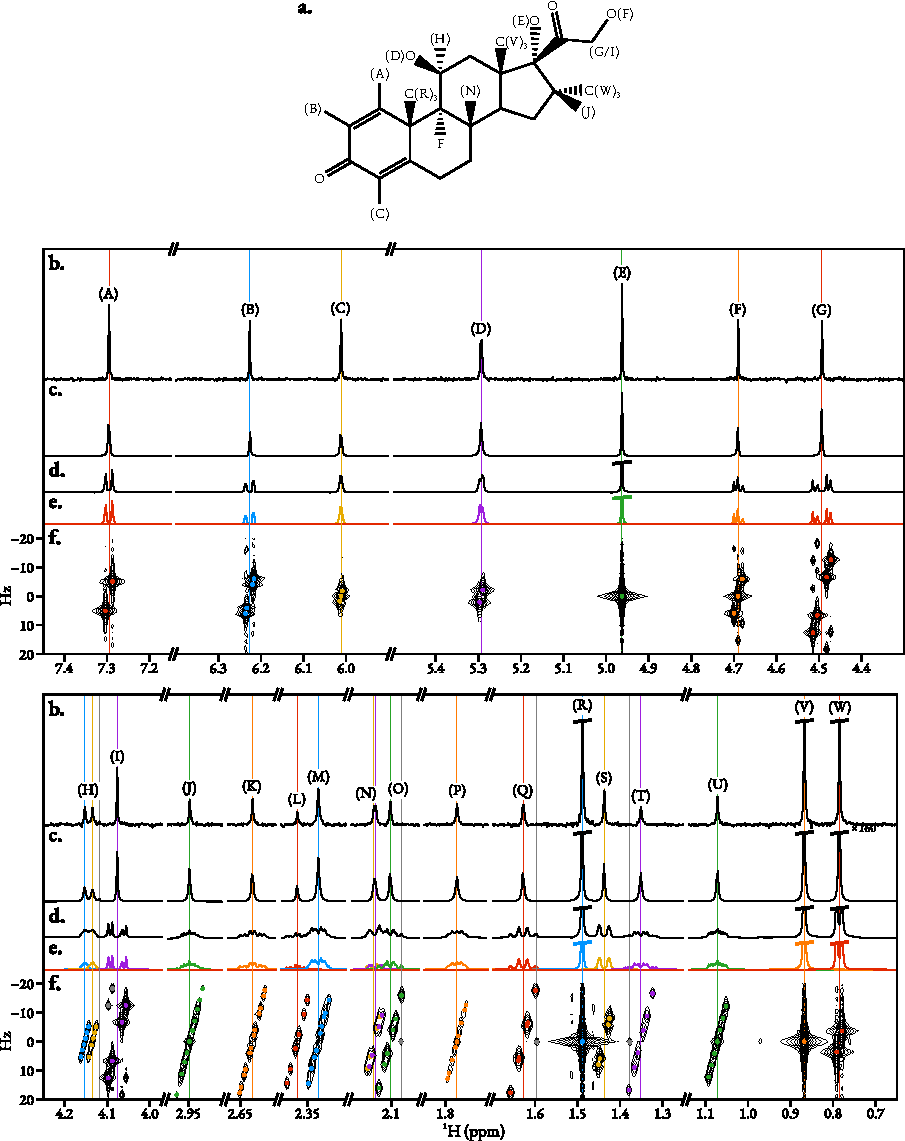
\includegraphics{dexamethasone_cupid/dexamethasone_cupid.pdf}%
    \caption[
        Application of \acs{CUPID} on a dexamethasone dataset.
    ]{
        \note{Fix magnification label.}
        Application of \acs{CUPID} on dexamethasone \ac{2DJ} dataset.
        \textbf{a.} \acs{TSE-PSYCHE} spectrum of the sample.
        \textbf{b.} The spectrum generated from \ac{FT} of the \ang{-45}
        signal.
        \textbf{c.} Conventional \acs{1D} spectrum.
        \textbf{.} Multiplet structures assigned ($\epsilon =
        \nicefrac{\fswtwo}{\Ntwo} \approx \qty{0.92}{\hertz}$).
        \textbf{d.} Contour plot of the absolute value mode \acs{2DJ} spectrum,
        with the locations of assigned oscillators given as coloured points.
    }
    \label{fig:dexamethasone-cupid}%
\end{sidewaysfigure}%
\note{Double check mp thold}

\subsection{Dexamethasone}


Figure \ref{fig:dexamethasone-cupid} shows the result of applying CUPID on a
dataset acquired from a sample dexamethasone in DMSO-d\textsubscript{6}. A
pure-shift spectrum was also acquired using the
\ac{TSE-PSYCHE} experiment\cite{Foroozandeh2018,Foroozandeh2015} for
comparison.
\ac{CUPID} generated a pure-shift spectrum with overall excellent agreement
with the \ac{TSE-PSYCHE} spectrum. Certain multiplet structures in the spectrum exhibit
splitting in the direct dimension, on account of heteronuclear couplings to
\textsuperscript{19}F. Most notable are those derived from spins (D), (H) \& (O). For the (D) multiplet, the
magnitude of the heterocoupling is very small such that assigning these to
separate oscillators was not achievable.
For the spin (N) multiplet, two separate structures were successfully assigned
(see the orange and green multiplets around \qty{2.1}{\partspermillion}).
The estimation routine was unsuccessful at accurately estimating the structure
associated with spin (H), where a severe under-fitting occurred. An under-fitting
of this structure even occurred when the estimation was re-run using
considerable over-estimation of the model order, with most oscillators in the
initial guess being purged during the \ac{NLP} procedure.
The spin (H) multiplet provides an extreme example line-broadening in the pure
shift spectrum on account of under-fitting. The most downfield peaks in the
CUPID spectrum (corresponding to aromatic and hydroxyl protons) also appear to
be noticeably broadened relative to their PSYCHE equivalents. This is also
probably due to under-fitting of the relevant multiplet structures, though to a
far less noticeable extent than for spin H. \note{Any other reason why this
might be so?}

\subsection{Estradiol}
\begin{figure}
    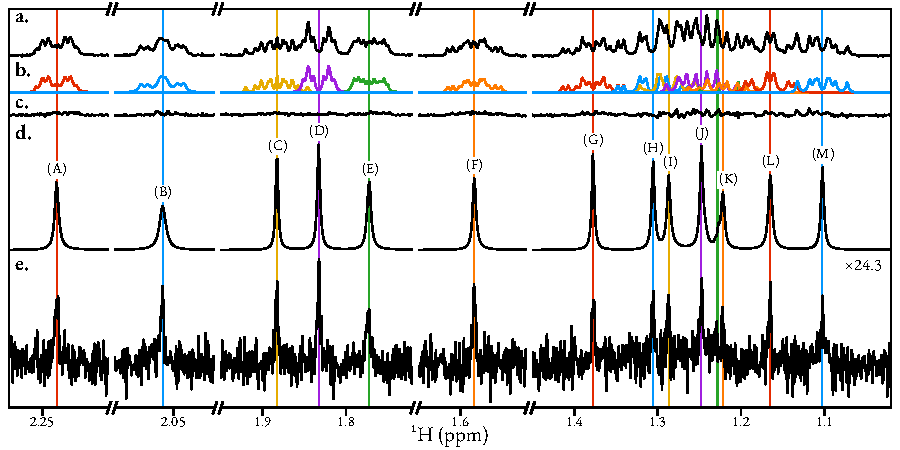
\includegraphics{estradiol_cupid/estradiol_cupid.pdf}%
    \caption[
        Application of \acs{CUPID} on a 17\textbeta-estradiol dataset.
    ]{
        Application of \acs{CUPID} on \ac{2DJ} dataset of 17\textbeta-estradiol
        in \acs{DMSOd6}.
        \textbf{a.} Spectrum of the first direct-dimension \ac{FID} in the
        \ac{2DJ} dataset.
        \textbf{b.} Multiplet structures assigned ($\epsilon =
        \nicefrac{\fswtwo}{\Ntwo} \approx \qty{2}{\hertz}$).
        \textbf{c.} The residual between the spectrum in panel a and the lines
        in panel b.
        \textbf{d.} The pure shift spectrum generated using \ac{CUPID}.
        \textbf{e.} \acs{PSYCHE} spectrum of the sample see Figure
        \ref{fig:psyche} for details on the pulse sequence. The spectrum has
        been scaled such that the maximum is of the same magnitude as the
        corresponding point in the \ac{CUPID} spectrum.
    }
    \label{fig:estradiol-cupid}%
\end{figure}

A final showcase of \ac{CUPID} is provided by Figure \ref{fig:estradiol-cupid}, where a low concentration (\qty{2}{\milli\molar}) sample of 17\textbeta-estradiol (Figure \ref{fig:structures}.

\section{Summary}
In this chapter, \ac{CUPID}, a procedure for the construction of pure shift
spectra via the holistic estimation of \ac{2DJ} datasets, is presented.
Such spectra can be possess myriad beneficial features relative to alternative
methods, albeit with the requirement of a complex post-processing procedure.

% The original method for pure shift spectrum generation consisted of shearing a
% magnitude-mode \ac{2DJ} spectrum by \ang{45}, and computing the projection onto
% the $\Ftwo$ axis. To overcome the grotesque lineshapes which arise due to the
% presence of dispersion character, and non-linearities in the magnitude-mode
% spectrum, severe data treatment such as the used of sine-bell apodisation are
% applied. The resulting pure shift spectra suffer from reduced intensities
% because of this. On top of this, the intensities of peaks are attenuated by
% different extents, such that relative peak integrals become meaningless. The
% presence of strong coupling in the spin system also introduces unwanted
% artefacts into the spectra.

% Experimental procedures  based on ``chunking'' the initial sections of the
% \acp{FID} in a \ac{2D} experiment\,---\,including \ac{ZS}, \ac{BIRD} and
% \ac{PSYCHE}\,---\,have largely superseded the shear and summation approach.
% One key disadvantage of all of these is that only a fraction of the available
% spin magnetisation contributes to the final pure shift spectrum, leading to
% poorer sensitivity.

Through a number of examples, it has been shown that by employing parametric
estimation, a simple \ac{2DJ} experiment can be harnessed to generate pure
shift spectra with sharp absorption Lorentzian peaks which retain the same
signal intensity as the \ac{2DJ} experiment. It it is able to perform
admirably even when state of the art techniques like \ac{PSYCHE} produce
spectra with such low \acp{SNR} as to render them unusable. Frequently, \ac{CUPID}
is able to automatically discard oscillators present in the model which either
correspond to strong coupling artefacts or noise, leading to simplified spectra
which appear to adhere to the weak coupling regime. There are cases where
strong coupling artefacts do end up in the estimation result. It has been shown
that these can be manually neglected from the parameter set so they don't have
an unwanted influence on final pure shift spectrum, though this requires manual
intervention from a knowledgeable user.

Simultaneously, \ac{CUPID} can assign multiplet structures,
by grouping oscillators which lie along a specific \ang{45} cross section in
frequency space. Achieving this experimentally\,---\,effectively involving
a \ac{2DJ} experiment in conjunction with a pure shift element\,---\,requires
running an extremely long (hours or even days) \ac{3D} pulse sequence. The
usefulness of the multiplet structures generated by \ac{CUPID} is dependent on
the level of the estimation routine's accuracy. On
numerous occasions within the examples presented here, the estimation routine
was unable to resolve certain, similar frequency signals. A complete
understanding of the coupling network associated with a given spin in not
attainable when this is so. However, such multiplet structures can still provide
valuable insights into the sample being studied.

\ac{CUPID} is limited by the complexity of the dataset of interest. The reasons
for this are two-fold. First, for datasets comprising progressively more peaks
in a given spectral region, the difficulty in generating effective parameter
estimates becomes harder. Second, with an increased model order required to
estimate the dataset, the time required for computation increases drastically.
This feature is most clearly observed when comparing the times required in
estimating the different regions considered in the estradiol example. As a rule
of thumb, it is anticipated that \ac{CUPID} will perform admirably on datasets
derived from small molecules, though datasets derived from large molecules such
as proteins are likely to be too complex and demanding for good results.

